\section{Method}
\label{sec:approach}

This section details our approach to discovering trace links in a software repository. Our approach takes a software repository and requirements as input and extracts trace links between requirements and the software issues, commits, and pull requests (PRs) by analyzing the textual fields of these artifacts. Our prototype tool visualizes the trace links and other information on the repository. Figure~\ref{fig:sys-flow} presents the main steps of our approach. We publicly share the implementation of our approach in our replication package\footnote{https://zenodo.org/record/8076982}

\begin{figure}[htb]
    \centering
    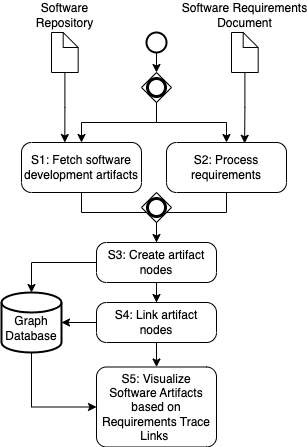
\includegraphics[width=0.65\linewidth]{figs/approach.png}
    \caption{Steps of our approach}
    \label{fig:sys-flow}
  \end{figure}

  The first two steps, \textsf{S1} and \textsf{S2}, concern processing the two inputs of our approach, a software repository and natural language requirements, respectively. \textsf{S1} fetches issues, pull requests, and commits from a repository whose URL is given. Our prototype expects a GitHub repository, however, our approach is general and can be applied to other repositories where the aforementioned development artifacts are present. %Table~\ref{tab:artifactfeatures} presents the attributes of these artifacts that are used in our approach.
  Our prototype expects a text file containing requirements. It does not enforce specific requirements and is able to process the requirements that are written in a hierarchical structure, which is a common practice.

          \begin{table}
        \centering
        \caption{Attributes of software development artifacts used in our approach}
        \label{tab:artifactfeatures}
        \begin{tabular}{lllll}
          \toprule
          & Requirement & Issue & PR & Commit \\
          \midrule
          ID &\checkmark &\checkmark&\checkmark&\checkmark\\
          Title &-&\checkmark&\checkmark&-\\
          Description &\checkmark&\checkmark&\checkmark&-\\
          URL&-&\checkmark&\checkmark&\checkmark\\
          Number&\checkmark&\checkmark&\checkmark&\checkmark\\
          State&-&\checkmark&\checkmark&-\\
          Creation Date&-&\checkmark&\checkmark&-\\
          Completion Date&-&\checkmark&\checkmark&\checkmark\\
          Message&-&-&-&\checkmark\\
          Comment Count&-&\checkmark&\checkmark&-\\
          Comment List&-&\checkmark&\checkmark&-\\
          Parent&\checkmark&-&-&-\\
          OID&-&-&-&\checkmark\\
          Text&\checkmark&\checkmark&\checkmark&\checkmark\\
          \bottomrule
        \end{tabular}
      \end{table}

 In \textsf{S3} nodes are created for each of the requirements, issues, pull requests, and commits. 
The features  in Table~\ref{tab:artifactfeatures} are added as the node attributes. 
 Our prototype uses Neo4j\footnote{https://neo4j.com} as a graph database.

      \textsf{S4}  links the requirements to artifacts by creating edges between their associated nodes. 
      Two types of relationships are captured between the artifacts, namely \emph{tracesTo} and \emph{relatedCommit}. 
      The  \emph{tracesTo} relationship represents a trace link between a requirement node and a software development artifact node. 
      The \emph{relatedCommit} is a relation between a commit and a pull request node. 
      This relation captures provides insight into how the commits are organized by the team. 
      In practice, requirements can trace directly to commits or via pull requests (as seen in Figure˜\ref{fig:rawtracegraph}).

      We implement and evaluate three methods to extract trace links, which are represented with the \emph{tracesTo} relation. 
 The first method extracts keywords from the requirements and development artifacts and links the requirements to the artifacts that share keywords. 
 The other methods are based on the \textit{term frequency-inverse document frequency} (TF-IDF) vectors and \textit{word vectors} obtained from a pre-trained model.
For these methods, requirements are linked to the artifacts with similar vectors. 
      The overview of the processing of software artifacts to extract the trace links is shown in Algorithm~\ref{alg:process-software-artifacts}.
            \makeatletter
\algnewcommand\algorithmicswitch{\textbf{switch}}
\algnewcommand\algorithmiccase{\textbf{case}}
\algnewcommand\algorithmicassert{\texttt{assert}}
\algnewcommand\Assert[1]{\State \algorithmicassert(#1)}%
% New "environments"
\algdef{SE}[SWITCH]{Switch}{EndSwitch}[1]{\algorithmicswitch\ #1\ \algorithmicdo}{\algorithmicend\ \algorithmicswitch}%
\algdef{SE}[CASE]{Case}{EndCase}[1]{\algorithmiccase\ #1}{\algorithmicend\ \algorithmiccase}%
\algtext*{EndSwitch}%
\algtext*{EndCase}%
\makeatletter

\setphaserulewidth{0.4pt}

\begin{breakablealgorithm}
\caption{Trace links graph construction}
\label{alg:process-software-artifacts}
\begin{algorithmic}[1]
\State Input: $RSD$ \Comment{Requirement Specification Document}
\State Input: $GRU$ \Comment{Github Repository URL} 
\State Input: $M$ \Comment{Trace Extraction Method} 
\State Input: $\tau_{e}$ \Comment{Threshold for Vector-Based Methods} 
\State Output: $TG$ : \texttt{graph} \Comment{Trace Graph}
\phase{Fetch Software Artifacts}
% \LineComment{Request from Github graphQL API}
\State $\textit{issueList} \hspace{-0.1cm} \leftarrow$  \hspace{-0.2cm} getIssues($GRU$)\label{algl:m}
\State $\textit{prList} \hspace{-0.1cm} \leftarrow$  \hspace{-0.2cm} getPRs($GRU$)\label{algl:m}
\State $\textit{commitList} \hspace{-0.1cm} \leftarrow$  \hspace{-0.2cm} getCommits($GRU$)\label{algl:m}
% \LineComment{Parse directly from given Requirement Specification Document}
\State $\textit{reqList} \hspace{-0.1cm} \leftarrow$  \hspace{-0.2cm} getRequirements($RSD$)\label{algl:m}

\phase{Create Graph with Artifacts}

  \Switch{$s$}
    \Case{$a$}
      \Assert{0}
    \EndCase
    \Case{$b$}
      \Assert{1}
    \EndCase
  \EndSwitch

% \State neo4jConnector($issue_nodes$)\Comment{}

\State $\textit{sdaList} \hspace{-0.1cm} \leftarrow$  \hspace{-0.2cm} $issueList+prList+commitList$\label{algl:m}
% \State $\textit{TG} \hspace{-0.1cm} \leftarrow$  \hspace{-0.2cm} $issueNodes+prNodes+commitNodes+reqNodes$\label{algl:m}
\State $TG \leftarrow$  \texttt{graph} 

\For{\textbf{each} $a$ \textbf{in} sdaList} \label{algl:c}
\State $TG$.addNode(a)
\EndFor \label{algl:c}

\For{\textbf{each} $r$ \textbf{in} reqList} \label{algl:c}
\State $TG$.addNode(r)
\EndFor \label{algl:c}

\phase{Extract Trace Links}

\State preprocess($reqList$, $method$)
\State preprocess($sdaList$, $method$)
\For{\textbf{each} $r$ \textbf{in} reqList}
\For{\textbf{each} $a$ \textbf{in} sdaList}
\If{$method=$ "keyword"}
\State $keywords \leftarrow$ extract(r)
\If{$a.text$ contains any $kw$ in $keywords$}
\State $TG$.addEdge(r,a)
\EndIf
\EndIf
\If{$method=$ "vector-based"}
\State r-v $\leftarrow$ createVector($r.text$)
\State a-v $\leftarrow$ createVector($a.text$)
\If{sim(r-v, a-v)  $\geq$ $\tau_{e}$}
\State $TG$.addEdge(r,a)
\EndIf
\EndIf
\EndFor
\EndFor

\Return $TG$
\end{algorithmic}

\end{breakablealgorithm}

The \textit{getIssues, getPRs, getCommits} functions take a project repository  ($GRU$) and make API calls to the GitHub API\footnote{\url{https://docs.github.com/en/graphql}} to fetch a list of issues, PRs, and commits respectively. 
It fetches the properties shown in Table \ref{tab:artifactfeatures} for these software software artifacts. 
The \textit{$preprocess(list, method)$}  function takes  a list of software artifacts and a method for trace link creation. 
It lemmatizes the text property of each artifact in the list. 
If the method is vector-based then it also removes the stopwords. 
Thereafter, the trace links are determined according to desired method.
In the keyword based method shared keywords between the requirements and software artifacts are sought. In vector based methods the requirements and artifacts are vectorized and their similarities are compared. When similarities exceed a given threshold edges are formed.
For vector-based methods we utilize TF-IDF and word vectors.


% The $sEdge(req, sda, method)$  function determines whether a trace link exists between a given a requirement ($req$) and a software development artifact ($sda$) based on a trace link $method$. If  $method$ is `keyword extraction', the keywords are extracted from $req$ and $sda$ and an edge is created if they share keywords.
% If  $method$ is `vector-based' (tf-idf or word-embedding) vectors are created for  $req$ and $sda$  using their text property. 
% Then, the similarity between the vectors are calculated. 
% An edge is created if similarity value is above a predefined threshold.

 The following details the trace extraction methods referred to in the algorithm. 

      \paragraph{Keyword Case} To identify the most relevant keywords of the requirements, the following NLP methods are utilized:  
      % We identify the keywords from the requirements as our trace link direction is from requirements to the software development artifacts.
      \begin{itemize}
      \item \textit{Tokenization}: Each requirement is tokenized to obtain its words.
      \item  \textit{Part-of-Speech Tagging}: Each word is categorized according to its part-of-speech (POS) tags. 
      This work specifically focuses on nouns and verbs when identifying relevant keywords. 

      \item  \textit{Dependency parsing}: The dependency trees of the requirement sentences are obtained using spacy\footnote{https://spacy.io/api/dependencyparser} .
      Figure~\ref{fig:deptree} shows a dependency tree for a requirement.
      The verbs and nouns that are related to objects via the direct object and the object of preposition relations are used to create \emph{verb-object} and \emph{noun-object} pairs.
      The remaining verbs and nouns are also captured.
      All of these are used to find the artifacts that are relevant to the requirements.

      \item  \textit{Stopword removal}: English stopwords are used to remove the singleton nouns and verbs which are not distinguishing.

      \item  \textit{Project stopwords removal}: Users are allowed to provide project-specific stopwords. 
      \end{itemize}

\begin{figure*}[htbp]
    \centering
    
\includegraphics[width=1\linewidth]{figs/displacy.png}
    \caption{The dependency tree of a requirement.}
    \label{fig:deptree}
  \end{figure*}

  Using these NLP tasks we identify the significant keywords from requirement specifications and prepare a base for identifying trace links. 
  Figure~\ref{fig:keywords} shows the extracted keywords for a given requirement.

  \begin{figure}[H]
    \centering
    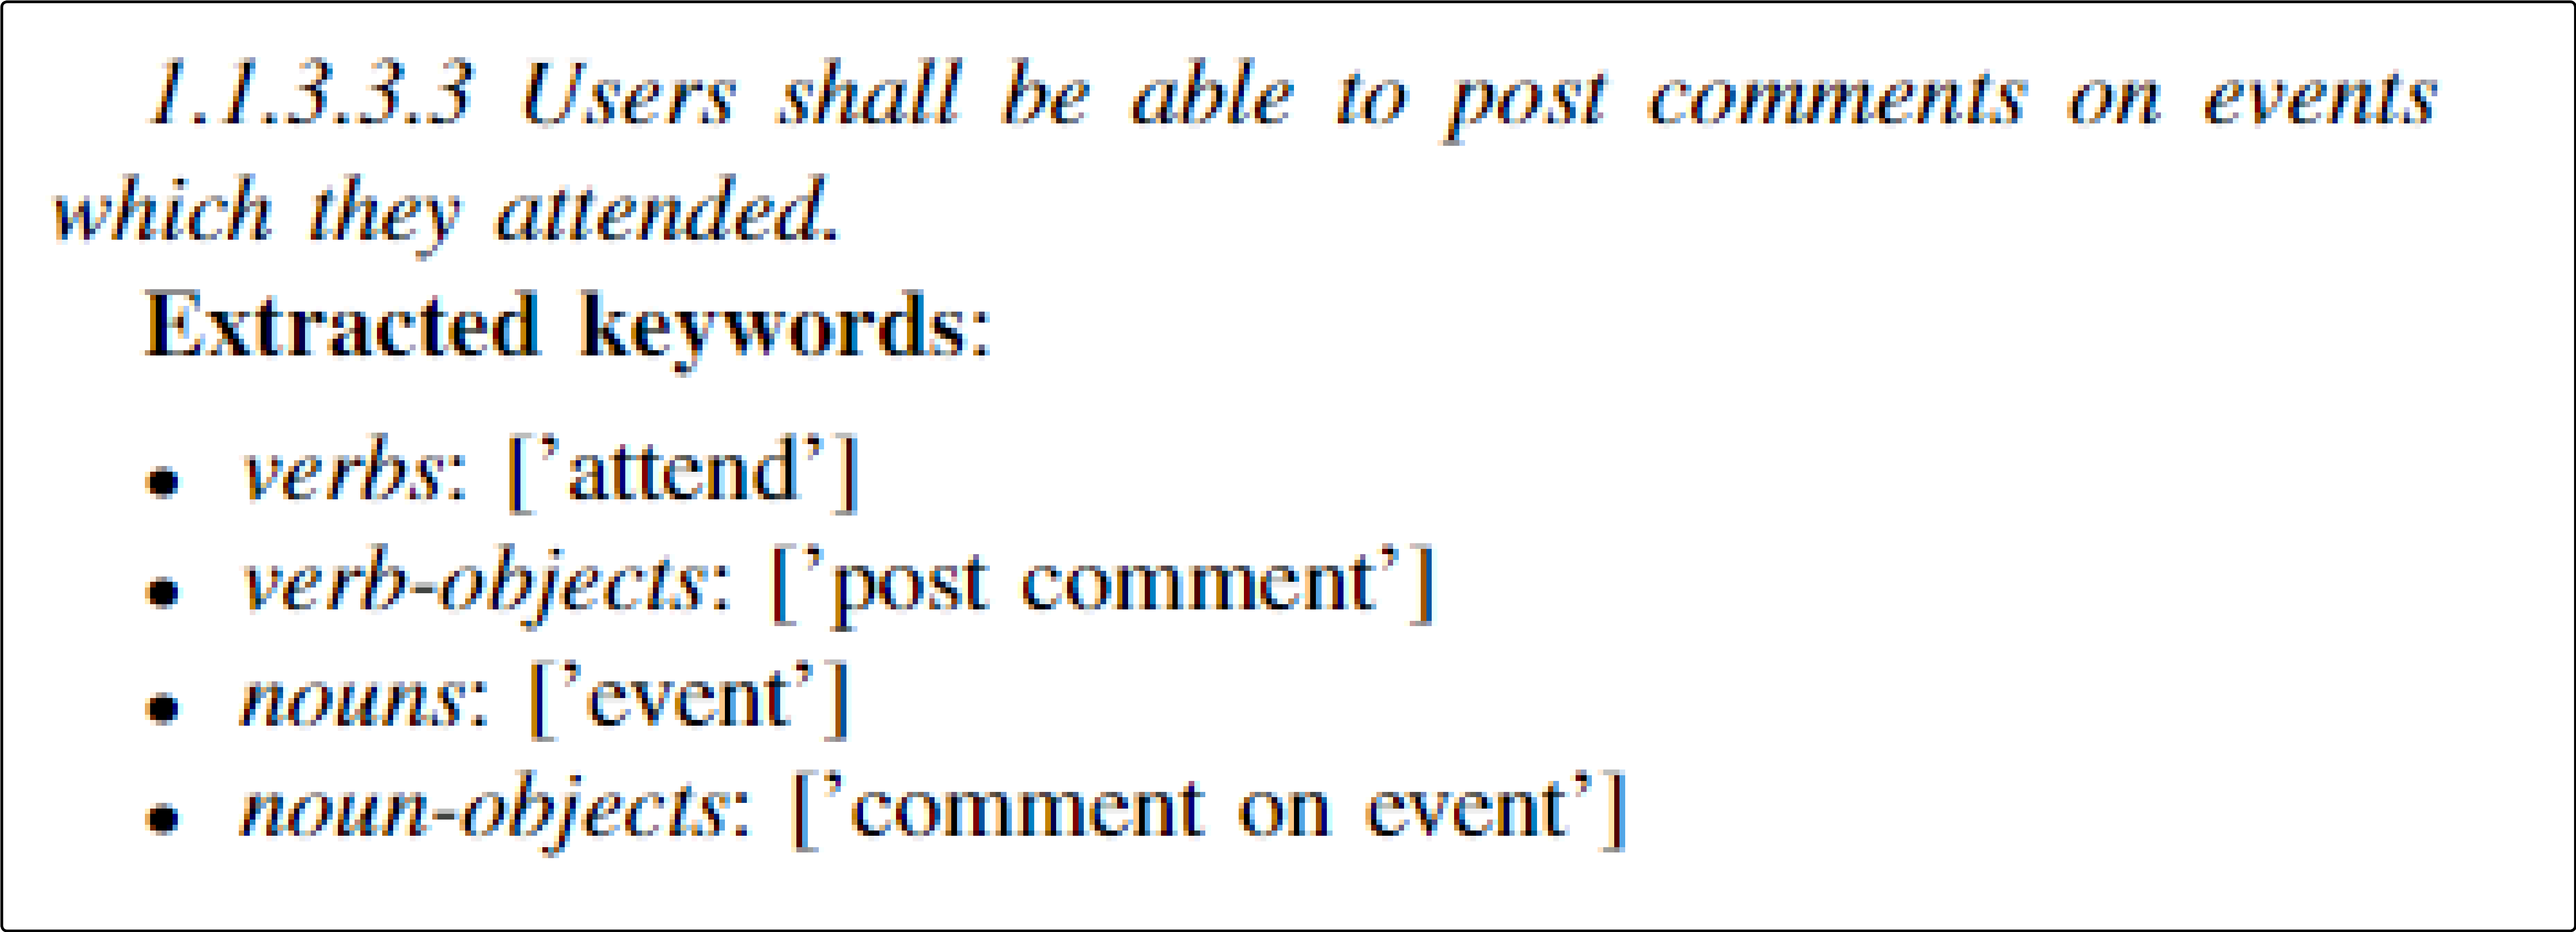
\includegraphics[width=.96\linewidth]{figs/keywords.png}
    \caption{Keyword extraction from a requirement.}
    \label{fig:keywords}
  \end{figure}

  The extracted keywords are matched against the textual attributes of the software artifacts to determine the trace links.
  These traces are stored in a graph database with the relation type \emph{tracesTo}.

  \paragraph{TF-IDF Vectors} Initially, a set of all the words in the requirements and the software development artifacts is created. 
  Stopwords are removed from this set, from which
  % TF-IDF values are computed using the  
  TF-IDF vectors are created for each requirement and artifact using equations \ref{eq:tf}, \ref{eq:idf}, and \ref{eq:tfidf}. 
  The requirements are linked with artifacts that have a similarity score above a given threshold (see Section~\ref{sec:eval}).
  Figure~\ref{fig:tfidfvec} presents the steps for this method.

  \begin{align}
    TF(t,d) &= \frac{\text{frequency of t in d}}{\text{total number of terms in d}} \label{eq:tf} \\
    IDF(t) &= log\frac{N}{1+df} \label{eq:idf}\\
    TF\text{-}IDF(t,d) &= TF(t,d)*IDF(t) \label{eq:tfidf}
  \end{align}

      \begin{figure}[H]
        \centering
        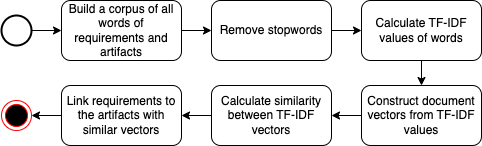
\includegraphics[width=0.95\linewidth]{figs/tfidfvector2.png}
        \caption{Steps for extracting trace links based on TF-IDF vectors}
        \label{fig:tfidfvec}
      \end{figure}

      \paragraph{Word Vectors} To generate a vector for each artifact, we use a pre-trained word embeddings model (word2vec-google-news-300 \footnote{\url{https://huggingface.co/fse/word2vec-google-news-300}}). 
      We represent requirements as the average of their word vectors. 

      Just like in TF-IDF method, cosine similarity is used to link requirements to artifacts.
      The artifacts that have similarities above a predefined threshold are considered to be linked. 
      % To extract trace links for a requirement using TF-IDF and word vectors, 
      % we calculate the cosine similarity metric of the requirement's vector with the vectors of other artifacts. 
      Figure~\ref{fig:wordvec} presents the steps of the word vector method.

       \begin{figure}[htb]
        \centering
        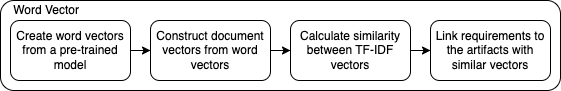
\includegraphics[width=0.99\linewidth]{figs/wordvector.png}
        \caption{Steps of trace link extraction based on word vectors}
        \label{fig:wordvec}
      \end{figure}



\begin{figure}[htb]
    \centering
    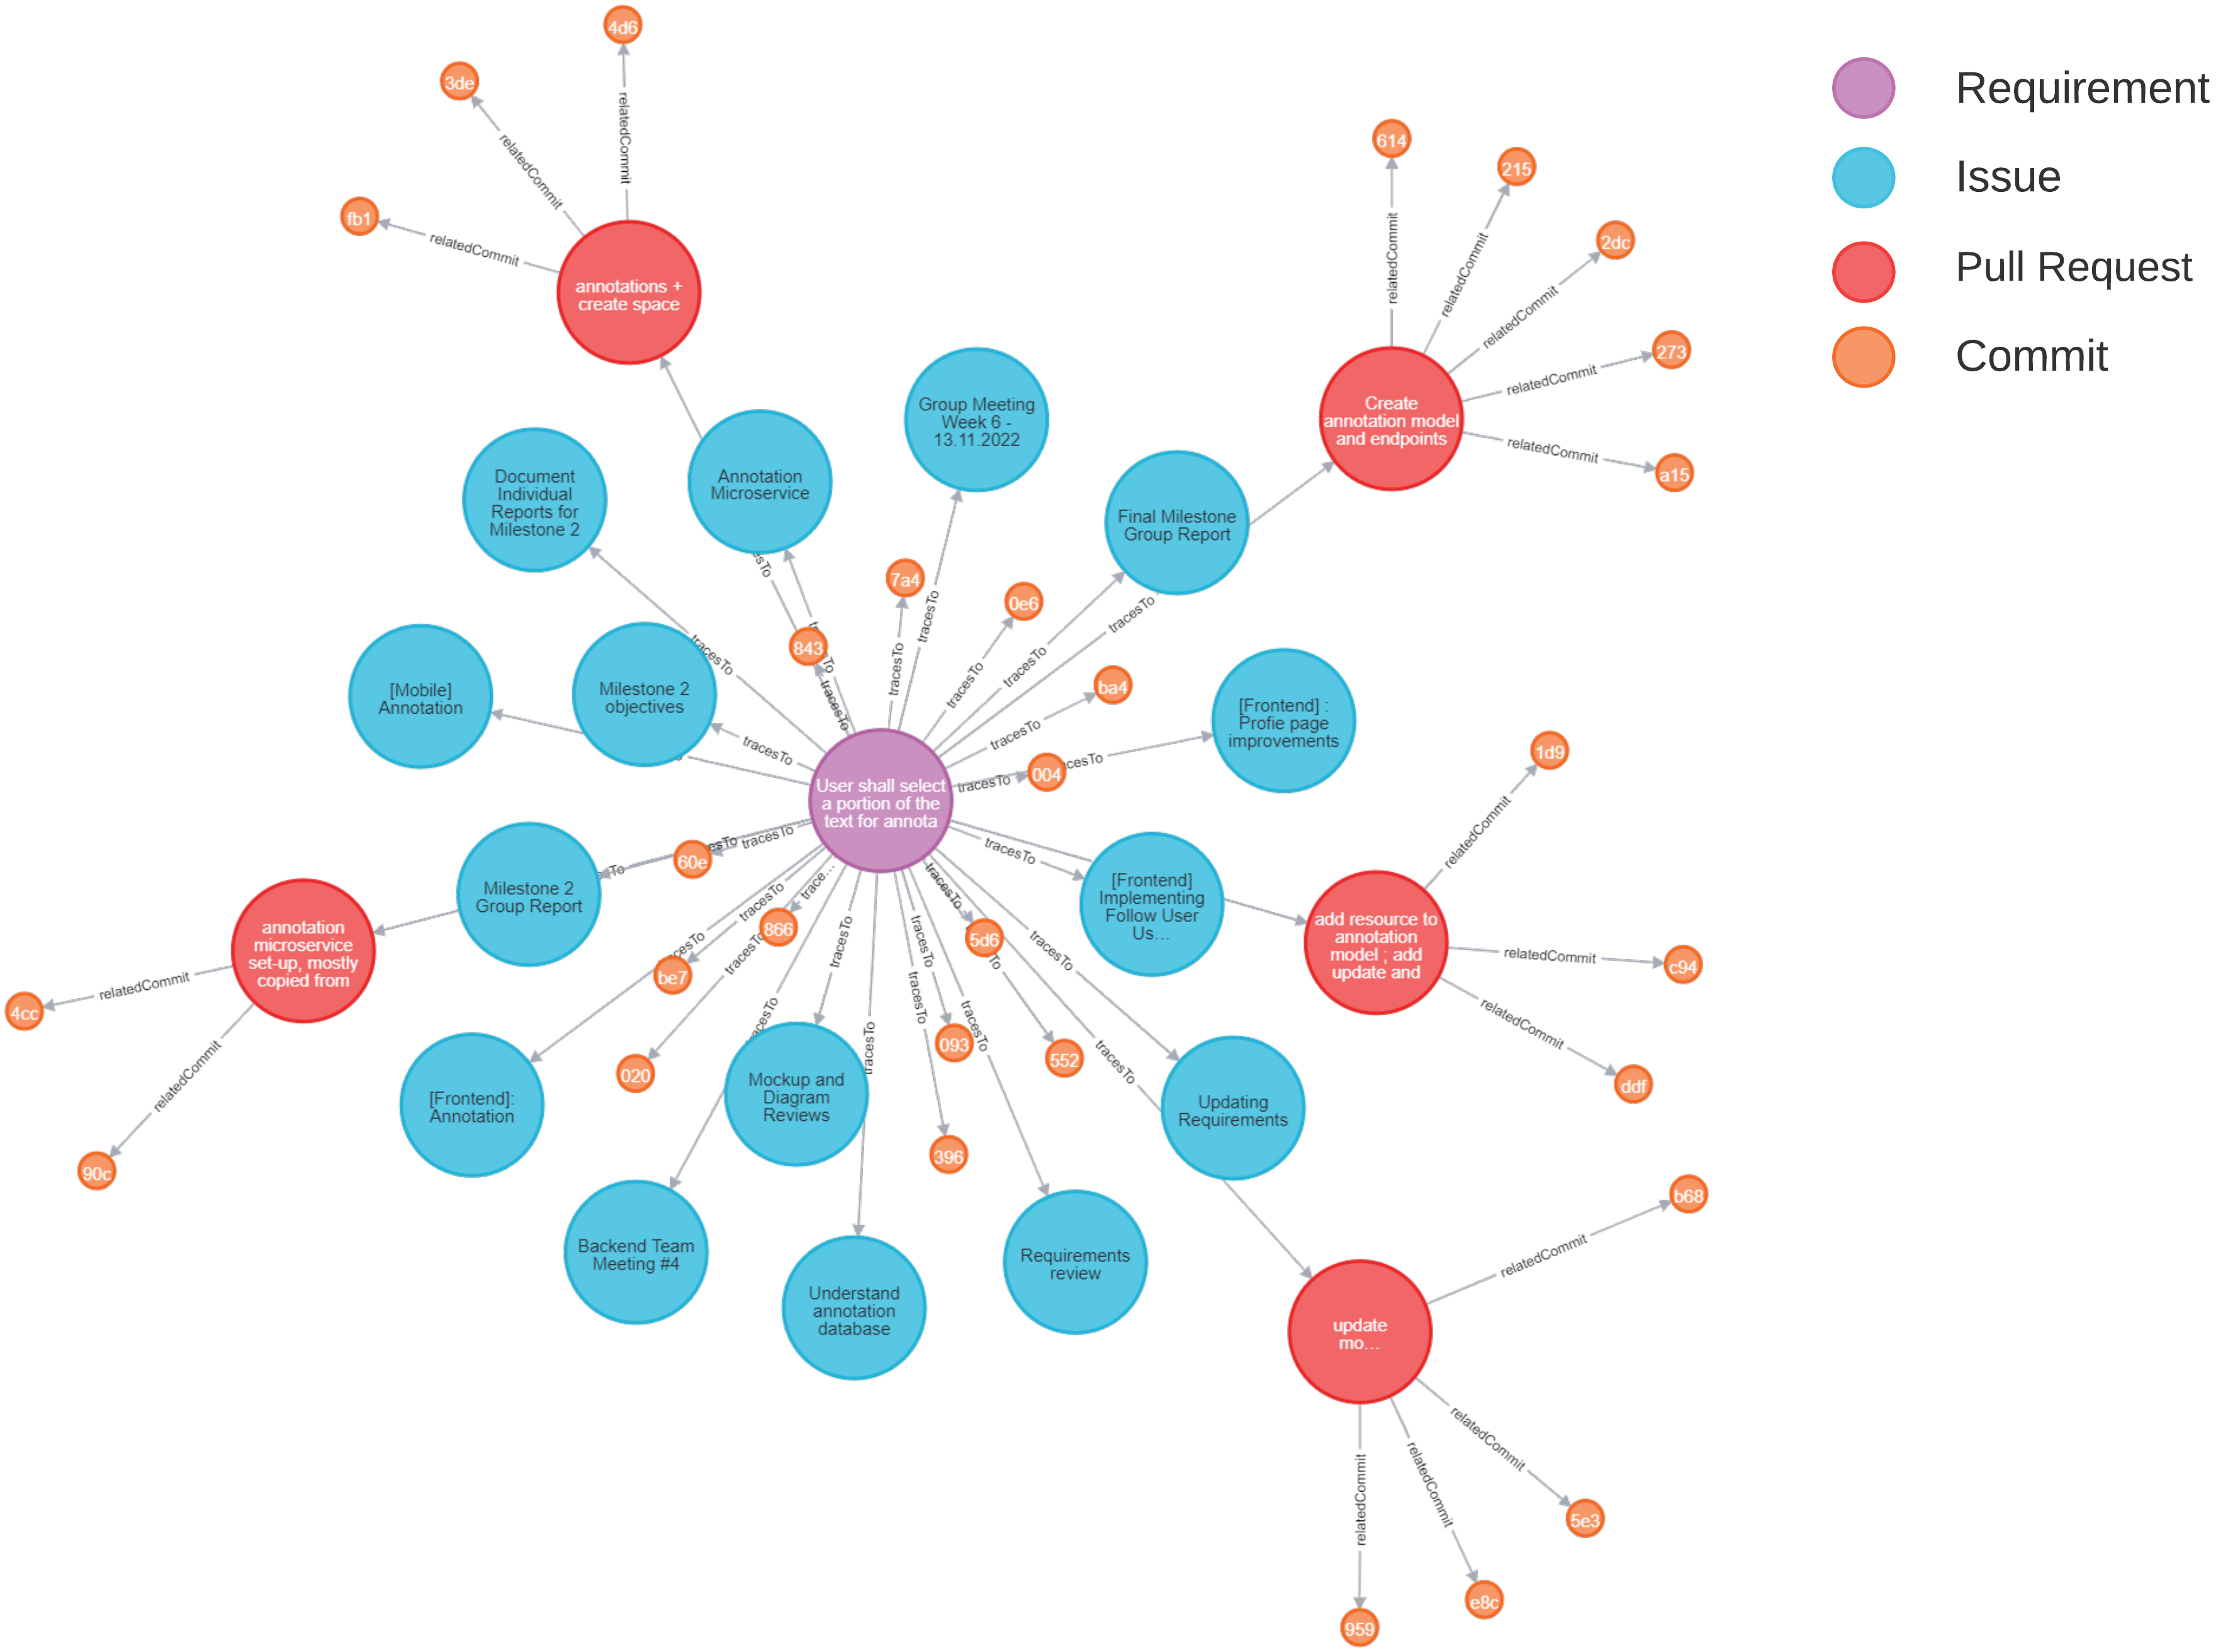
\includegraphics[width=1\linewidth]{figs/rawTraceGraph.png}
    \caption{A segment of a trace graph.}
    \label{fig:rawtracegraph}
  \end{figure}

  The obtained trace links are added to the trace graph with the \emph{tracesTo} edge type. 
  The relations between pull requests and commit nodes are stored with the \emph{relatedCommit} edge type.
  Figure~\ref{fig:rawtracegraph} illustrates a segment of a trace graph of a requirement.

\begin{figure}[htb]
    \centering
    
\includegraphics[width=.99\linewidth]{figs/traceGraph.png}
    \caption{A segment of a trace graph on a time axis.}
    \label{fig:tracegraph}
\end{figure}

The trace graph  not only visualizes the software development artifacts (SDA)  traced from requirements, but it also can display the lifetime of the activities over time. 
Figure~\ref{fig:tracegraph} shows the SDAs related to a requirement which are arranged along a time axis based on their \textit{creationDate} property. 
Here, we see that first pull request related to the requirement was created in week 8, while the issues concerning the planning of the requirement were created in the early stages of the development. 
Such visualization is useful during the development phase of software projects as well as a while performing retrospective analyses.




% - The requirement to be examined is the root.
% - The requirement is connected to its related SDAs with \textit{tracesTo} links.
% - Pull request nodes have related commit nodes connected with \textit{relatedCommit} link.

% Who looks at trace?\\
% Trace graph can help a project manager or a developer
% Why?\\
% What can be found?


% A project manager looking at the trace graph can identify:

% \begin{itemize}
%     \item The planning phase of this requirement goes back to week 1
%     \item The implementation of this feature started at week 8
%     \item This requirement took around 13 weeks of work??
%     \item ...
% \end{itemize}

% \pagebreak

% Or in the case of a problem or a bug related to annotation, for example, a developer can view the trace of the requirement about annotation, localizing the search for the problem. Lets say the problem is about updating annotations. Looking at the trace graph, an educated guess can be made, with the information about the problem, to look at a specific pull request. For example, in our case user can view \textit{"Create annotation model"} and \textit{"... add update and delete annotation endpoints..."} nodes. Both nodes can be further observed by using the url property, reaching the github page and examining the code related to them.



Finally, \textsf{S5} provides a visualization where the user can browse the software development artifacts based on the trace links. 
We report several types of information extracted from the repository to support software development project management. 
Neodash\footnote{\url{https://neo4j.com/labs/neodash/}} is integrated into our Neo4j graph database to provide an interactive dashboard to explore the trace graph.

The dashboard presents information about a software repository and enables exploration based on trace links.
First, an overview of the software artifacts for a software repository.  
The number of issues and pull requests is visualized in a stacked bar chart per week to view the project's progress over time. 
Similarly, the number of  issues closed per week is visualized with a stacked bar chart. 
The dashboard also shows the total number of open/closed issues, open/merged PRs, and the average number of trace links per requirement. 
These statistics serve as a snapshot of the current state of the project. 
Figure~\ref{fig:barcharts} shows the dashboard for a repository.

\begin{figure}[hbt]
    \centering
    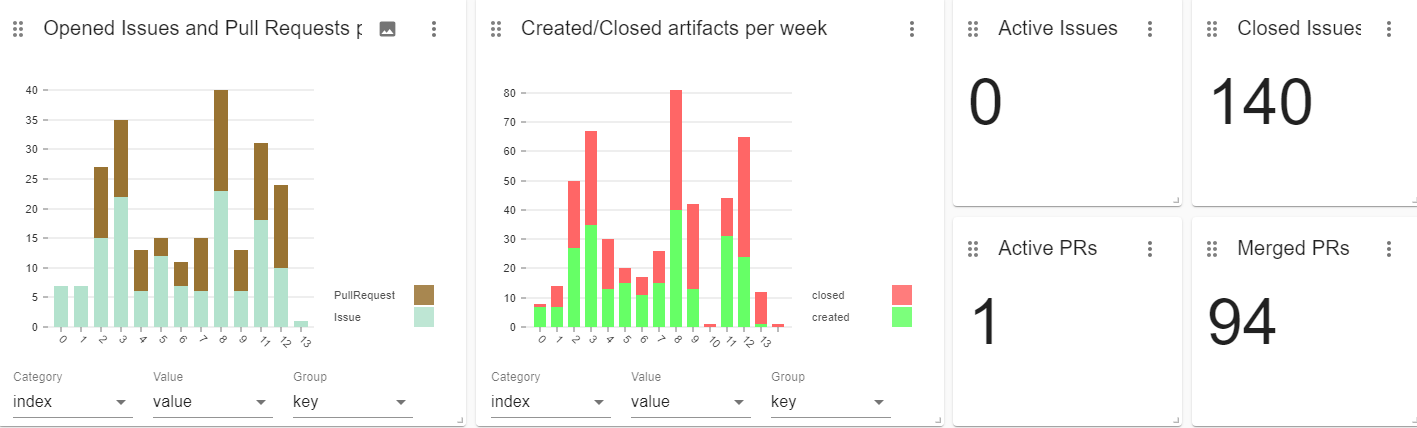
\includegraphics[width=.9\linewidth]{figs/dashboard-barcharts.png}
    \caption{Information about the software artifacts of a project. The first bar chart shows the weekly issues and pull requests created. The second bar chart shows opened and closed artifacts per week.  On the right, is the total number of currently active issues and PRs and completed tasks (issues and PRs). }
    \label{fig:barcharts}
\end{figure}

The dashboard displays the trace links for a requirement over the course of the project on a weekly basis to track the progress of a requirement.
It is presented using a line chart as shown in Figure~\ref{fig:linechart}. 
The project manager can visualize the data of a single requirement or compare the progress of multiple requirements. 
This comparison allows the users to observe the effort associated with each requirement
since it displays the number of software development artifacts traced to them.

\begin{figure}[htb]
    \centering
    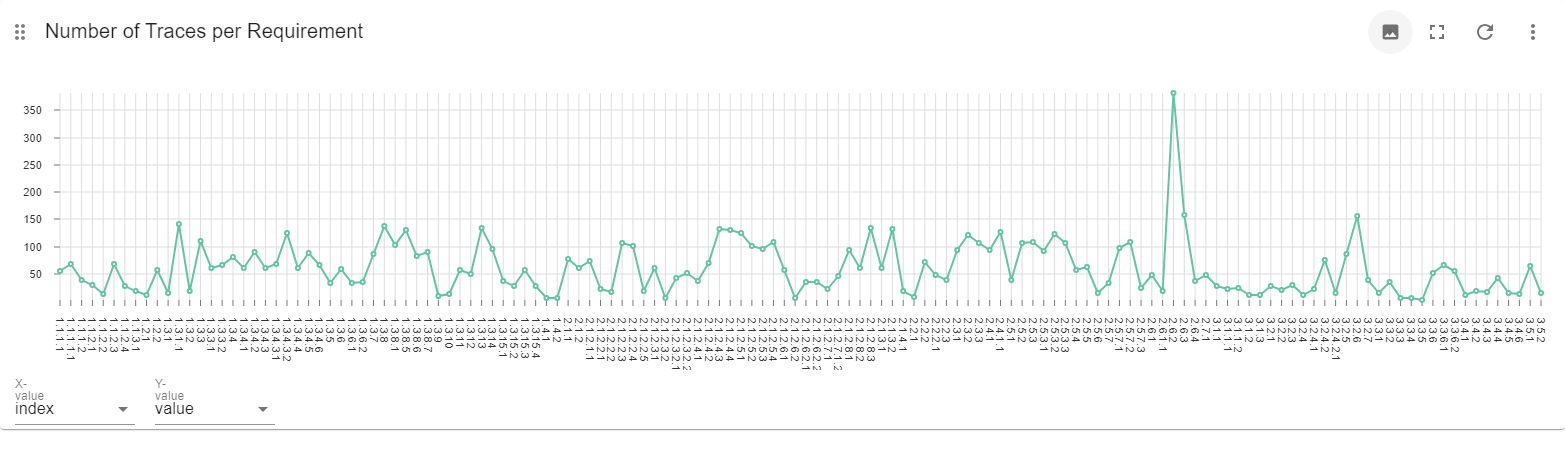
\includegraphics[width=.9\linewidth]{figs/linechart.png}
    \caption{The number of trace links for each requirement. }
    \label{fig:linechart}
\end{figure}

The dashboard shows a comparative  view of two requirements with their weighted relations to software artifacts using  a Sankey diagram (Figure~\ref{fig:sankey}).
Here, thicker lines represent a stronger relation between the requirements to their traced artifacts. 
Thus, one can see how requirements are related via their associated software artifacts.

\begin{figure}[htb]
    \centering
    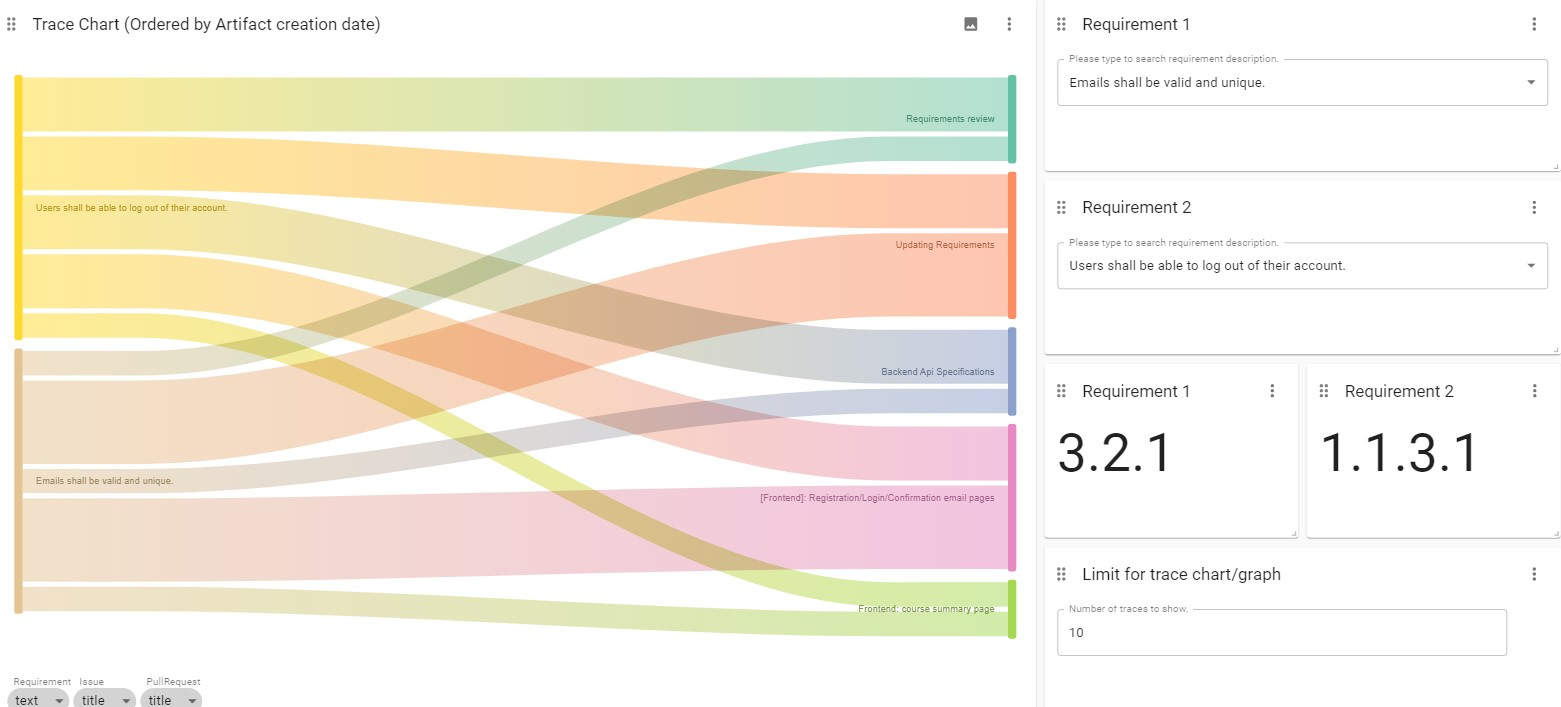
\includegraphics[width=.9\linewidth]{figs/sankey.jpg}
    \caption{The weighted relations between requirements and their associated software artifacts.}
    \label{fig:sankey}
\end{figure}

Users can interact with the dashboard to gain insights on selected requirements as seen in Figure˜\ref{fig:perreq}. 
The identified traces are presented in graphical and tabular formats for  selected requirements.
Their  current status and weekly activities are displayed in the last section of the dashboard.

\begin{figure}[htb]
    \centering
    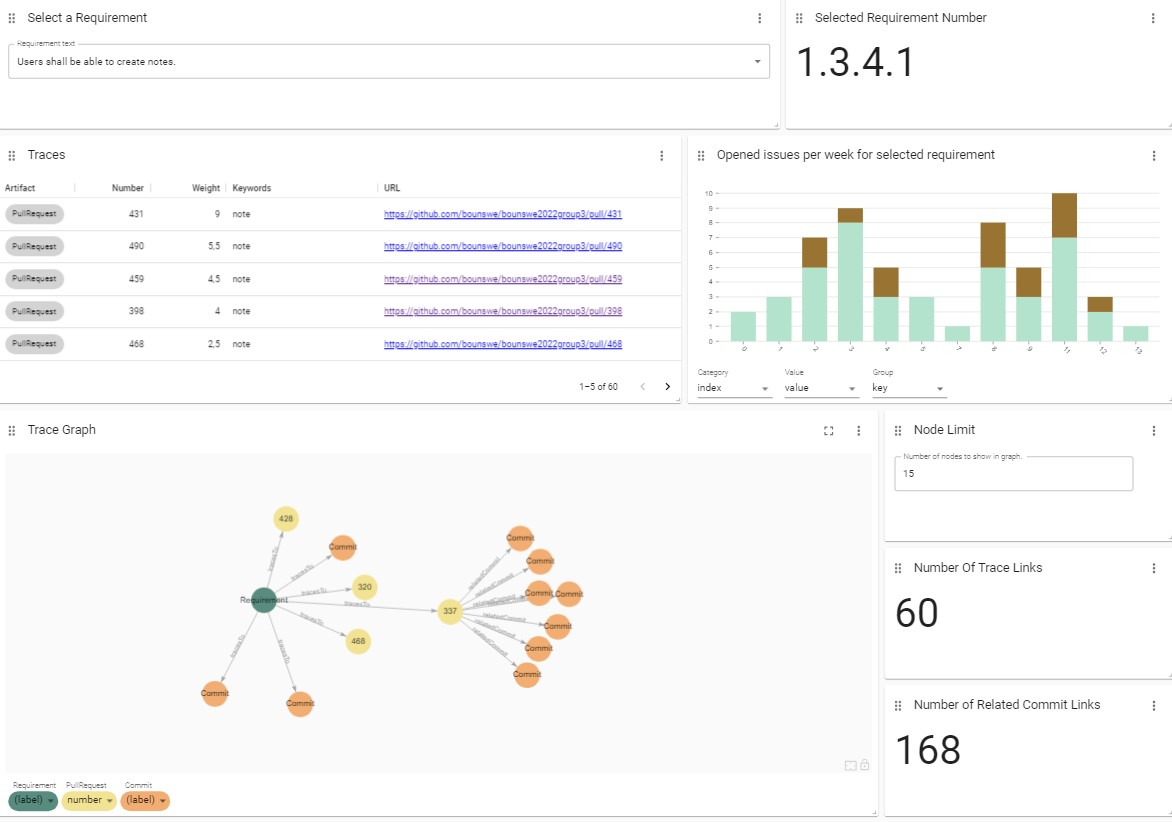
\includegraphics[width=.9\linewidth]{figs/perreq.jpg}
    \caption{Detailed information about a selected requirement.}
    \label{fig:perreq}
\end{figure}

